
%----------------------------------------------------------------
%
%  File    :  open_source.tex
%
%  Authors :  ???
% 
%  Created :  7 Sept 2019
% 
%  Changed :  7 Sept 2019
% 
%---------------------------------------------------------------

\section{Open Source Lösung}
\label{sec:open_source}

Im Vergleich zu teurer Spezial-Hardware und nicht frei zugänglicher Software, gibt es auch sogenannte Open-Source Lösungen. Grundsätzlich kann eine Software als Open-Source bezeichnet werden, wenn der Quellcode dieser veröffentlicht wird. Im Gegenzug, zur einfachen Bereitstellung einer rein ausführbaren Datei.
Des Weiteren wird frei zugängliche Software oftmals mit eingeschränkten, oder keinen Beschränkungen weitergegeben. Diese ist daher oftmals frei und kostenlos zu verwenden und somit auch erweiter- und veränderbar \cite{gacek2004many}. 

Allerdings gibt es nicht eine einzige Lizenz, unter welche Open-Source Software zur Verfügung gestellt wird. Dabei unterscheiden sich diese teils gravierend. So ist es beispielsweise erlaubt, Änderungen an einer, unter der Berkeley Software Distribution (BSD) Lizenz veröffentlichten Software, Änderungen vorzunehmen und diese unter eine beliebige, auch nicht freie Lizenz, zu stellen. Lediglich der Vermerk auf die Ursprüngliche Lizenz muss vorhanden bleiben. Wohin gegen die GNU General Public License (GPL) besagt, dass eine veränderte Software, welche bereits und der GPL veröffentlicht wurde, ebenfalls unter die GPL zu stellen ist, also wieder frei zugänglich und veränderbar sein muss. Es gibt aber auch noch weitere Open-Source Lizenzen, wie etwa: Apache License, Common Public License (CPL), Mozilla Public License (MPL), European Public License (EUPL), MIT License uvm \cite{rosen2005open}.

\subsection{OpenAirInterface - OAI}
Im konkreten Anwendungsfall, ermöglicht uns eine solche Software, kostengünstig ein eines eigenes LTE-Netzwerk aufzubauen. 
Ganz ohne Hardware geht dies natürlich nicht, jedoch würde ein Modul für etwa 1500 Dollar ausreichen um ein funktionsfähiges Netz aufzubauen. Ein solches Software Defined Radio (SDR) ist das "Flexible, next-generation, open source software-defined radio" von LimeMicrosystems, welches im Zuge einer Crowdfunding-Aktion realisiert wurde \cite{CroudLime01}. 
LimeMicrosystems hat eine große Community und hat es sogar bereits geschafft, ihren limeSDRs in Satelliten zu verbauen \cite{limeHp}. 

Mit einem SDR werden Anteile der Signalverarbeitung mittels Software realisiert. Dies kann von dedizierter Hardware unterstützt werden. Des Weiteren bietet es eine gewisse Flexibilität zu einer reinen Hardwarelösung, da Software veränderbar ist \cite{jondral2005software}. 

Das OpenAirInterface ist ein Projekt der OpenAirInterfaceTM Software Alliance (OSA), welches eine Open Source Lösung zur Verfügung stellt \cite{OpenAir19}.

Dabei wird die Lösung in zwei Projekte unterteilt. 
\begin{itemize}
	\item eNodeB (eNB): “openairinterface5G”
	\item evolved packet core (EPC): “openair-cn”
\end{itemize}

OpenAirInterface ist die erste LTE Open-Source Software Platform, welche den vollen Protokollstack des 3GPP Standards, inklusive E-UTRAN und EPC unterstützt.
Dabei wird dies sowohl für das Erstellen eines eigenen LTE Netzes, als auch das Überwachen(Monitoring) verwendet \cite{nikaein2014openairinterface}.
Des Weiteren ist es möglich Performance-Analysen durchzuführen und dabei Einblick zu erhalten, wie sich ein rasch skalierendes System verhält. 

\begin{figure*}[ht]
	\centering
	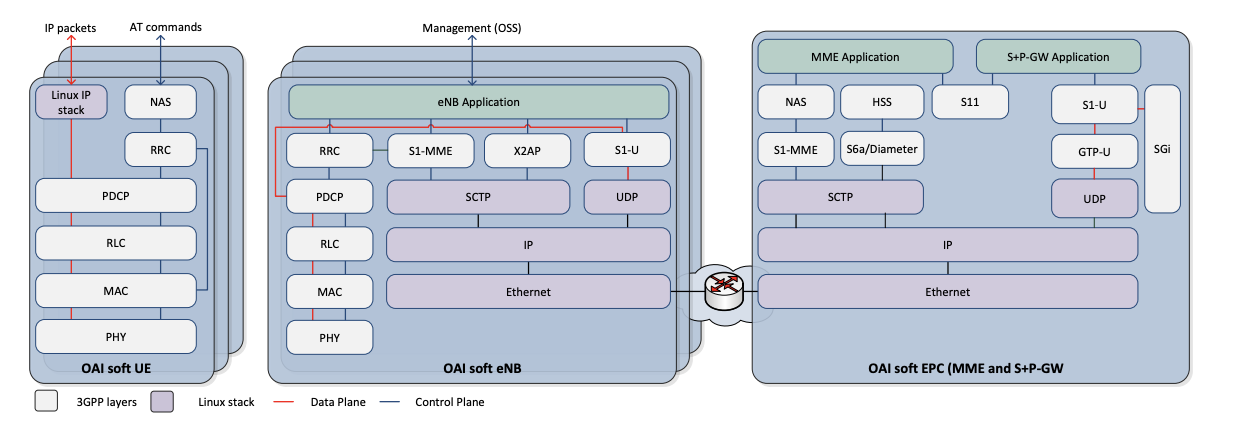
\includegraphics[width=1.025\linewidth]{BestandTeileOAI}
	\caption{Übersicht LTE Module in den jeweiligen Projekten \protect\cite{openAirInterfaceOverview19}}
	\label{fig:modulesOAI}
\end{figure*}


Abbildung \ref{fig:modulesOAI} zeigt die schematische Implementierung des LTE Protokoll Stacks in OAI.
Dem Hersteller zufolge wurden hiermit auch diverse Tests durchgeführt. So wurde Beispielsweise OAI eNB mit kommerziellen Huawei Geräten getestet, bei welchen LTE aktiviert wurde (E392, E398u-1) und OAI-UE mit CMW500 (Ericsson on com4Innov network)

Die OpenAirInterface Open.Source Initiative bietet sowohl Unterstützung für eNodeB, UE wie auch EPC an. Zudem wird, neben dem oben erwähnten LimeSDR, auch noch Universal Software Radio Peripheral (USRP™) der Firma Ettus und ExpressMIMO2 unterstützt. Des Weiteren erlaubt OAI hierbei auch die Unterstützung kommerzieller Ausrüstung \cite{kaltenberger2019openairinterface}. Somit ist man hier nicht auf ein spezielles SDR eingeschränkt.

\subsection{srsLTE}
srsLte bietet eine sehr modulare Architektur, um auch rasch neue Standards einfließen lassen zu können. Die Architektur ist in funktionale Module aufgebaut. Zudem wird hiermit bereits ein Satz an Beispielanwendungen geboten, welche für eigene Anwendungen angepasst werden können \cite{puschmann2017implementing}. 
Des Weiteren sind auch Anpassungen möglich, um zusätzliche Hardware zu unterstützen. 
Abbildung \ref{fig:modulessrsLTE} zeigt diesen modularen Aufbau.

\begin{figure*}[ht]
	\centering
	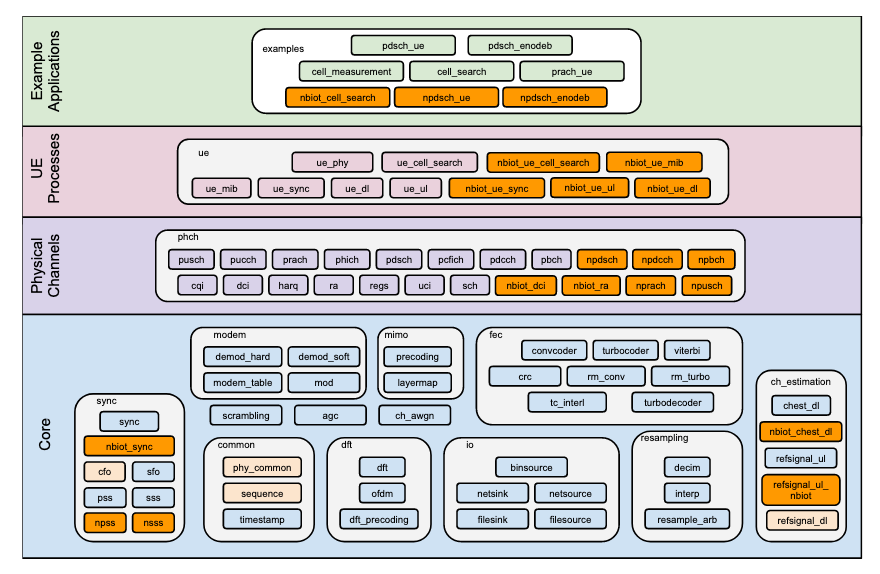
\includegraphics[width=1.015\linewidth]{ssrLTE_Module}
	\caption{Übersicht Architektur srsLTE \protect\cite{puschmann2017implementing}}
	\label{fig:modulessrsLTE}
\end{figure*}

Die Beispielanwendungen geben einen Überblick zum Betrieb als eNodeB (srsENB, srsEPC) sowie Informationen, um dies als UE (srsUE) einsetzen zu können. Entwickelt wurde dies von Software Radio Systems, welche dieses Projekt auf Github zur Verfügung stellt \cite{githubSrSLTE}.

Die hohe Flexibilität und Anpassbarkeit ist auch ein Grund dafür, dass srsLTE als Basis für andere Projekte und Anwendungen eingesetzt wird. So ist etwa \nameref{tinyLTE} eines dieser genannten Projekte. Zudem wird die Software regelmäßig gewartet, was auch an den Codeänderungen im Repository zu erkennen ist. 

\subsection{tinyLTE}
\label{tinyLTE}
Eine weitere Open-Source Lösung ist tinyLTE. Auch diese verwendet das Prinzip des SDR, um größtmögliche Flexibilität und Offenheit zu bieten. Dabei unterstützt tinyLTE sowohl den Betrieb als LTE Client (UE) wie auch als Infrastruktur (eNodeB + EPC) \cite{eckermann2018tinylte}.

Der Vorteil dabei ist, dass hiermit ein gleichzeitiger Betrieb, sowohl als Sende- wie auch als Empfangseinrichtung möglich ist. In Kombination mit Hardware, welche 2 SDRs bietet, kann so, ein einzelnes Gerät die volle Funktionalität von LTE bieten. 
Beides basiert, mit geringen Änderungen, auf srsLTE \cite{gomez2016srslte}. 

Die Lösung von Philipp Gorczak sowie Fabian Eckermann, wurde auf Github zur Verfügung gestellt. Eine Evaluierung im Betrieb wurde ebenfalls bereits getestet. Dabei ging es um die Kommunikation mittels LTE zwischen Fahrzeugen \cite{tinyLteGithub}. 

\subsection{Unterschiede}
Alle drei erwähnten Lösungen bieten einen breiten Funktionsumfang und Unterstützung an. Unterschiede sind etwa in der getesteten Hardware zu erkennen. Sollte bereits bestehendes Equipment vorhanden sein, könnte dies ein Indikator für eine Präferenz darstellen. 
tinyLTE wurde speziell für die Kommunikation zwischen Fahrzeugen entwickelt und getestet. 